\section{Building TextGNN on Agent-Data Graphs}
\label{sec:text-gnn}

\xhdr{TextGNN motivations}
The agent-data graph $\mathcal{G}$ provides a platform for expressing a complex multi-agent scenario, \eg, a human research community.
To further simulate based on a given real-world agent-data graph, we need agentic models, \eg, LLMs, to generate new data and interactions on the agent-data graph.
To this end, motivated by the message-passing algorithm in GNNs, we proposed a text-based message-passing mechanism on an agent-data graph, called \textit{TextGNN}, where all hidden states are defined in the text space instead of the embedding space.



\xhdr{Recap: message passing in standard GNN} 
In standard GNNs, input features $\mb{x}_v$ are used to initialize the initial states $\mb{x}_v = \mb{h}_v^{(0)}$. Afterward, the goal is to learn useful node embeddings \( \mb{h}_v \) by iteratively aggregating information from local neighborhoods. Hidden states, message functions, and aggregation functions are the three main components in one GNN layer. The \( k \)-th iteration of message passing (or the \( k \)-th GNN layer) is typically defined as:

\begingroup
\small
\begin{equation}
    \label{eq:gnn}
    \mb{m}_u^{(k)} = \textsc{MSG}^{(k)}(\mb{h}_u^{(k-1)})
\end{equation}
\endgroup
\begingroup
\small
\begin{equation}
    \label{eq:gnn2}
    \mb{h}_v^{(k)} = \textsc{AGG}^{(k)}\big(\mb{h}_v^{(k-1)}, \{\mb{m}_u^{(k)} \mid u \in \mathcal{N}(v)\}\big)
\end{equation}
\endgroup
where \( \mb{h}_v^{(k)} \) is the node embedding at the \( k \)-th layer, \( \mb{h}_v^{(0)} = \mb{x}_v \) is the initial node feature, and \( \mathcal{N}(v) \) is the set of neighbors of node \( v \). \(\textsc{MSG}^{(k)}(\cdot)\) is a transformative function to convert the hidden states of one node into a message for aggregation. \(\textsc{AGG}^{(k)}(\cdot)\) is defined to update the hidden states of a node based on neighborhood messages. More generally, we can broadly consider the $k$-th layer of GNN to be an aggregation function that implicitly includes message functions inside:

\begingroup
\small
\begin{equation}
\mb{h}_v^{(k)} = \textsc{AGG}^{(k)}\big(\mb{h}_v^{(k-1)}, \{\mb{h}_u^{(k-1)} \mid u \in \mathcal{N}(v)\}\big)
\end{equation}
\endgroup

\begin{figure*}[t]
    \centering
    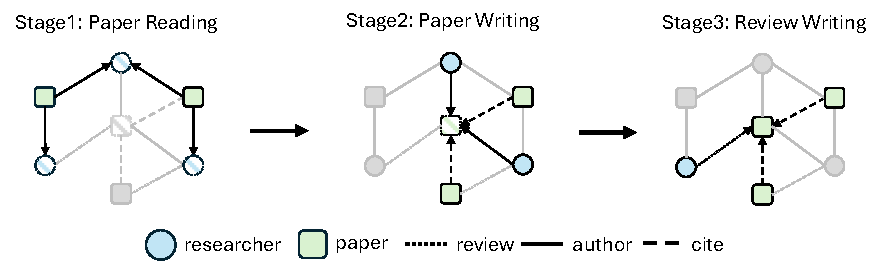
\includegraphics[width=0.82\linewidth]{./figs/community_activity.pdf}
    \caption{\textbf{\envname simulation as TextGNN inference on the community graph}. The simulation proceeds in three stages: (1) paper reading, where new agent nodes are added based on existing data; (2) paper writing, where data nodes are created; (3) review writing, where the community evaluates and selectively removes (or retains) generated nodes.}
    \label{fig:community-activity}
    \vspace{-2mm}
\end{figure*}


\xhdr{Message passing in TextGNN} Following the message-passing process in the standard GNN, we now define a general form of the aggregation function to describe the text-based message-passing process on an agent-data graph $\mathcal{G}$. The key difference between a standard GNN and a TextGNN is that all hidden states in the standard GNN are defined in the embedding space ($\mb{h}_v \in \mathbb{R}^d$) while those in TextGNN are defined in the text space ($\mb{h}_v \in \Sigma^{*}$). In a TextGNN, we first set the initial hidden states for data nodes $\mb{h}_v^{(0)} = \mb{x}_v$, where $\mb{x}_v$ are text attributes, and the initial hidden states for agent nodes is empty $\mb{h}_u^{(0)} = \emptyset$. Next, we design a general form of message passing function that handles three distinctive types of interaction, including agent-agent $\mathcal{E}_{aa}$, agent-data $\mathcal{E}_{ad}$, and data-data $\mathcal{E}_{dd}$.

Specifically, the $k$-th TextGNN layer for an agent node $u\in \mathcal{V}_a$ can be written as:
\begingroup
\small
\begin{equation}
\begin{aligned}
    \mb{h}_{u}^{(k)} &= \textsc{AGG}^{(k)}\big(f_u(\cdot), \mb{h}_u^{(k-1)}, \{\mb{h}_d^{(k-1)} \mid (u,d) \in \mathcal{E}_{ad}\}, \\
    &\quad \{f_a(\cdot), \mb{h}_a^{(k-1)} \mid (u,a) \in \mathcal{E}_{aa}\}\big) \\
    &= f_u\Big(\Big[\mb{h}_u^{(k-1)}, \big\{f_a\big(\big[\mb{h}_a^{(k-1)}, \mb{h}_u^{(k-1)}, \mb{h}_d^{(k-1)}\big]\big) \mid \\
    &\quad (u,a) \in \mathcal{E}_{aa}, (u,d) \in \mathcal{E}_{ad}\big\}\Big]\Big)
\end{aligned}
\label{agg_agent}
\end{equation}
\endgroup
where $[\cdot]$ is the concatenation function between texts to fill in the prompt template, $\mb{h}_v^{(k)}$ represents the hidden states of the $k$-th layer of $v\in \mathcal{V}$, $f_a(\cdot)$ represents the agent function paired with the agent node in the neighborhood and $f_u(\cdot)$ represents the agent function paired with the agent node.


Similarly, the forwarding process of the $k$-th TextGNN layer for a data node $v\in \mathcal{V}_d$ can be written as:
\begingroup
\small
\begin{equation}
\begin{aligned}
    \mb{h}_{v}^{(k)} & = \textsc{AGG}^{(k)}\Big( \mb{h}_v^{(k-1)}, \{\mb{h}_d^{(k-1)} \mid (v,d) \in \mathcal{E}_{dd}\}, \\
    &\quad \{f_a(\cdot), \mb{h}_a^{(k-1)} \mid (v,a) \in \mathcal{E}_{ad}\}\Big) \\
    &= f_g\Big(\Big[\mb{h}_v^{(k-1)}, \big\{f_a\big(\big[\mb{h}_a^{(k-1)}, \mb{h}_v^{(k-1)}, \mb{h}_d^{(k-1)}\big]\big) \mid \\
    &\quad (v,a) \in \mathcal{E}_{ad}, (v,d) \in \mathcal{E}_{dd}\big\}\Big]\Big)
\end{aligned}
\label{agg_data}
\end{equation}
\endgroup
where $f_g(\cdot)$ is defined as a global agent function without a specialized profile, and $f_a(\cdot)$ is the agent function paired with the agent node in the neighborhood.


